\documentclass[a4paper, 11pt, toc=listof, toc=bib, twoside=off]{scrbook}

% Quelle: https://www.fh-swf.de/media/neu_np/fb_in/professorinnen_3/giefers/pub/docs/LaTeX-Vorlage_Abschlussarbeit.zip
% Vorlage fuer Abschlussarbeiten
% Version 2022-05-17
% Getestet mit TeX Live; Kodierung: UTF8

% Hier Daten eintragen:
\newcommand{\name}{Jonas Michel Berger}
\newcommand{\abschlussarbeit}{Bachelorarbeit}
\newcommand{\hochschule}{Fachhochschule Südwestfalen}
\newcommand{\datum}{1. Oktober 2022}
\newcommand{\titeldeutsch}{Entwicklung eines Telegram-Bots zur Abfrage von Informationen aus der Software Graylog per Sprachnachricht}
\newcommand{\titelenglisch}{Development of a Telegram Bot to Retrieve Information From Graylog Software via Voice Message}
\newcommand{\erstpruefer}{Prof. Dr. Hans-Georg Eßer}
\newcommand{\zweitpruefer}{Prof. Dr. Heiner Giefers}
% Ende der Daten

\usepackage[inner=25mm, outer=25mm, top=25mm, bottom=25mm]{geometry}
\usepackage[utf8]{inputenc}
\usepackage[T1]{fontenc}
\usepackage{lmodern}
\usepackage[ngerman]{babel}
\usepackage[style=alphabetic, backend=biber, citestyle=ieee, bibstyle=numeric]{biblatex}
\addbibresource{literatur.bib}
\usepackage{csquotes}
\MakeOuterQuote{"}
\usepackage{scrlayer-scrpage}\lohead{\rightmark}\rehead{\leftmark}\ohead{\pagemark}
\usepackage{booktabs}
\usepackage{microtype}
\usepackage{graphicx}
\usepackage{scrhack}
\usepackage{hyperref}
\parindent0pt\parskip6pt

\usepackage{listings}
\renewcommand{\lstlistingname}{Listing}
\renewcommand{\lstlistlistingname}{Listingverzeichnis}
\lstset{basicstyle=\small\ttfamily, breaklines=true, numbers=left}
\lstset{literate=%
    {Ö}{{\"O}}1
    {Ä}{{\"A}}1
    {Ü}{{\"U}}1
    {ß}{{\ss}}1
    {ü}{{\"u}}1
    {ä}{{\"a}}1
    {ö}{{\"o}}1
    {~}{{\textasciitilde}}1
}

\linespread{1.15}

\graphicspath{ {./img/} }

\begin{document}
\frontmatter
\begin{titlepage}
\begin{center}
\begin{center}

\includegraphics{01_Logo-CMYK}
\end{center}

\vspace*{10mm}
\huge
\textbf{\titeldeutsch}

\vspace{10mm}
\Large
\titelenglisch

\vspace{15mm}
\LARGE
\textsc{\abschlussarbeit}

\vspace{20mm}
\large
\name

\hochschule

\datum
\end{center}
\end{titlepage}

\clearpage

\normalsize\normalfont

\thispagestyle{plain}
\begin{tabular}{ll}
Autor: & \name \\
Referent: & \erstpruefer \\
Korreferent: & \zweitpruefer \\
Eingereicht: & \datum
\end{tabular}

\chapter*{Zusammenfassung}
\addcontentsline{toc}{chapter}{Zusammenfassung}

Das Thema dieser Abschlussarbeit ist die Entwicklung eines virtuellen Assistenten (Bot) für den Telegram Messenger, welcher Netzwerkadministratoren bei ihrer täglichen Arbeit durch die Möglichkeit unterstützen soll, in Echtzeit Informationen zu ihrem verwalteten Netzwerk abrufen zu können. Dabei wird auf die Software Graylog zurückgegriffen, welche die zentrale Verwaltung von anfallenden Systemprotokollen für ein Netzwerk übernimmt. Der Systemadministrator kann vordefinierte Abfragen in der Bot-Software hinterlegen und verknüpfen, sodass diese auf Anfrage jederzeit an die in Graylog integrierte Suchmaschine übermittelt werden können.

\chapter*{Erklärung}

Ich erkläre hiermit, dass ich die vorliegende Arbeit selbstständig verfasst und dabei keine anderen als die angegebenen Hilfsmittel benutzt habe. Sämtliche Stellen der Arbeit, die im Wortlaut oder dem Sinn nach Werken anderer Autoren entnommen sind, habe ich als solche kenntlich gemacht. Die Arbeit wurde bisher weder gesamt noch in Teilen einer anderen Prüfungsbehörde vorgelegt und auch noch nicht veröffentlicht.

\bigskip
\noindent
\datum

\vspace{25mm}

\noindent
\name

\tableofcontents

\mainmatter
\ofoot*{}
\chapter{Einleitung}

Unternehmen haben heutzutage einen großen Anspruch an eine IT-Umgebung, welche möglichst fehler- und unterbrechungsfrei funktioniert. Um den Status der Geräte und Systeme in einem Firmennetzwerk bestmöglich überwachen und somit Fehler frühzeitig erkennen zu können, stehen den Systemadministratoren zahlreiche Werkzeuge zur Verfügung, welche die Überwachung auf Fehlerzustände eigenständig übernehmen und den Verantwortlichen somit eine mühselige und monotone Arbeit ersparen. Für die Überwachung der Systeme werden häufig zwei verschiedene Systeme verwendet: ein klassisches Monitoring-System überwacht im festgelegten Sekunden- oder Minutentakt einzelne Systeme auf ihre Erreichbarkeit und Funktionsfähigkeit. Weiterhin können im Monitoring Zustände wie der Füllungsgrad der Datenspeicher oder die Auslastung von CPU- und Arbeitsspeicherressourcen überwacht werden. Das Monitoring-System sorgt so für eine Überwachung der Betriebszustände der Systeme rund um die Uhr. In vielen Netzwerken wird zusätzlich ein Logserver eingesetzt, welcher die anfallenden Systemprotokolle der Geräte im Netzwerk zentral aufnimmt und durchsuchbar macht. Jede Software besitzt eine Art von Fehlerausgabe, welche je nach Einsatzzweck in das zentrale Systemprotokoll des Betriebssystems oder eine Textdatei geschrieben wird. Im Zeitalter von virtualisierten Umgebungen und Microservices hat sich die Anzahl der eigenständigen Systeme in einem Firmennetzwerk vervielfacht. Häufig werden Dienste in die Cloud ausgelagert, da dort Ressourcen und Kosten besser skaliert werden können. Fällt nun ein Dienst aus und es soll die Ursache ermittelt werden, können die Protokolle vom Logserver bezogen werden. Der Logserver bietet damit den weiteren Vorteil, dass Zusammenhänge besser sichtbar werden, da die Protokolleinträge der verschiedenen Systeme nebeneinander angezeigt werden. 

Das Produkt Graylog Open stellt Administratoren eine quelloffene und kostenlose Lösung zur Verfügung, welche eine Vielzahl von Schnittstellen für die Anbindung an Systeme in einem Netzwerk bietet. Für die Bedienung von Graylog und den Zugriff auf die erfassten Protokolle steht eine HTTP-Webschnittstelle für den Webbrowser zur Verfügung. Weiterhin bietet das Produkt eine REST-API für den programmgesteuerten Zugriff an. Mit dieser Schnittstelle können vielseitige benutzerdefinierte Lösungen entwickelt werden, wie eine Aufbereitung der Daten mittels Diagrammen oder der Anschluss der Software an ein Self-Service Portal. In Graylog können Regeln zur Aufbereitung der erfassten Daten definiert werden. So können spezifische Informationen wie HTTP-Statuscodes eines Webservers oder spezielle Schlüsselwörter mittels regulären Ausdrücken zum Zeitpunkt der Erfassung gefiltert und mittels Attributen global durchsuchbar gemacht werden.

\section{Ziel der Bachelorarbeit}

Es soll die Entwicklung eines Bots für den Telegram-Messenger in der Programmiersprache Python geplant und durchgeführt werden. Der Bot interagiert mit dem Benutzer über gesprochene Sprache indem der Anwender als Administrator eines Netzwerks die gewünschten Informationen zu Systemen im Netzwerk in einer Sprachnachricht beschreibt und der Bot mit einer per Sprachsynthese erstellte Nachricht antwortet. Die Informationsquelle ist eine Installation des Logservers Graylog Open. Es wird vorausgesetzt, dass die Software bereits für den Betrieb im Firmennetzwerk eingerichtet wurde und sämtliche zu überwachende Systeme angeschlossen wurden. Der Anwender kann beispielsweise Informationen zu Webservern im Firmennetzwerk anfordern: "Liefere mir Informationen zu Fehlern bei Webservern im Zeitraum der letzten 24 Stunden". Der Bot soll nun die Inhalte der Nachricht in eine Anfrage an die in Graylog integrierte Suchmaschine umwandeln und dem Anwender das Ergebnis aufbereitet wiedergeben, z.B.: "Es wurden 30 Ereignisse gefunden". Zu den Aufgaben der zu entwickelnden Software gehört die Koordination der Ereignisse inklusive der Behandlung von Fehlerfällen sowie die Kommunikation mit dem Benutzer.

\section{Aufbau der Bachelorarbeit}

Im Anschluss an dieses Kapitel werden die technischen Grundlagen erläutert. Hierzu zählen insbesondere die verwendeten Produkte und eine genauere technische Erläuterung, wie die Systeme in der zu entwickelnden Software zusammenarbeiten. Im dritten Kapitel wird die Planung der Software erläutert. Dabei wird auf Modelle des Softwareengineering zurückgegriffen sowie der Programmablauf mit UML-Diagrammen erläutert. Schließlich werden Entscheidungen erläutert, welche bei der Planung getroffen wurden. Im vierten Kapitel wird die Implementierung behandelt. Das Kapitel startet mit der Beschreibung der Einrichtung der Softwareentwicklungsumgebung und der Implementierung erster funktionaler Prototypen. Außerdem werden Konzepte erläutert, welche zum Zeitpunkt der Umsetzung der Theorie in die Praxis erstellt wurden. Das fünfte Kapitel handelt von dem Einsatz der Software in der Praxis. Im sechsten Kapitel erfolgt eine Zusammenfassung und ein Ausblick auf mögliche technische Optimierungen.
\chapter{Grundlagen}

In diesem Kapitel werden die für die Entwicklung benötigten verwendeten technischen Grundlagen erläutert.

\section{REST}

REST ist eine Abkürzung für Representational State Transfer und wurde von Roy Fielding in seiner Dissertation aus dem Jahr 2000 \cite{rest} definiert. Es handelt sich hierbei um eine Auflistung von Eigenschaften und Anforderungen, welche durch eine REST-API erfüllt werden sollen. REST-APIs werden für viele Dienste des Internets meist unsichtbar für die Anwender für die Kommunikation zwischen informationstechnischen Systemen verwendet. In der englischen Sprache wird häufig das Adjektiv 'RESTful' für Ressourcen verwendet, welche die REST-Prinzipien anwenden.

\subsection{Anwendung in der Praxis}

Heutzutage stellen viele Dienste HTTP-APIs zur Verfügung, welche als 'RESTful' bezeichnet werden können. Die Kommunikation mit den Programmierschnittstellen beschränkt sich dabei auf das HTTP- und HTTPS-Protokoll, welches ebenfalls für den Abruf von Webinhalten im Browser verwendet wird. Durch die hohe Verbreitung wird die Implementierung neuer vernetzter Applikationen für Softwareentwickler stark vereinfacht. Das ursprünglich von Tim Berners-Lee entworfene Konzept des World Wide Web als Hypermedium wird so ebenfalls unterstützt. Ein Hypermedium beschreibt eine Ansammlung von Informationen (beispielsweise Websiten, welche im Quellcode vorliegen) mit Verweisen auf andere Informationen in dieser Menge. Bei in der Beschreibungssprache HTML (Hypertext Markup Language) geschriebenem Quellcode im World Wide Web handelt es sich um Hypertext mit Verweisen auf andere Medien (beispielsweise Quellcode anderer Webseiten; Audio-, Video- oder Bilddaten). 

Der Zugriff auf HTTP-APIs erfolgt analog zum Zugriff auf Webseiten im Internet. Je nach Anforderung werden die HTTP-Methoden \lstinline{GET}, \lstinline{POST} und weitere verwendet. Die von der HTTP-API beziehbaren Informationen werden mit der URL (Uniform Resource Locator) lokalisiert und angefordert. Zusätzlich können Informationen über Header (Kopfzeilen) und Cookies ausgetauscht werden, um beispielsweise Zustandsinformationen (Status des Warenkorbs in einem Webshop, Identifikationsnummer des angemeldeten Benutzers) austauschen zu können.

\begin{lstlisting}[caption={Beispiel eines Aufrufs der Graylog REST-API.}, label=bsp-rest-api]
GET http://10.10.12.1:9000/api/cluster

{
  "12ac8e44-0c59-4c38-bd5e-4fe247a55893": {
    "facility": "graylog-server",
    "codename": "Noir",
    "node_id": "12ac8e44-0c59-4c38-bd5e-4fe247a55893",
    "cluster_id": "8421ad08-fe62-4a04-8576-a81cab1a9c55",
    "version": "4.3.6+36120cf",
    "started_at": "2022-09-10T23:15:05.435Z",
    "hostname": "graylog.home.arpa",
    "lifecycle": "running",
    "lb_status": "alive",
    "timezone": "Europe/Berlin",
    "operating_system": "Linux 5.4.0-125-generic",
    "is_processing": true
  }
}
\end{lstlisting}

Die Antwort der HTTP-API erfolgt in vielen Fällen maschinenlesbar in der Sprache JSON.

\section{Telegram Messenger}

Der Dienst Telegram bietet seinen Nutzern eine Möglichkeit um kostenlos miteinander u.A. über Apps für die Mobilbetriebssysteme Android und iOS zu kommunizieren. Telegram hatte nach nach eigenen Angaben weltweit im Juni 2022 erstmals über 700 Millionen monatliche Nutzer und befand sich unter den fünf Apps mit den höchsten Downloadzahlen \footnote{\url{https://telegram.org/blog/700-million-and-premium}}. Der Dienst stellt damit eine beliebte Alternative zu anderen Messengern wie WhatsApp oder Signal dar. Ein Alleinstellungsmerkmal von Telegram gegenüber Whatsapp oder Signal sind die Bots und die dazugehörige API.

\subsection{Bots}

Der Begriff Bot stammt von dem englischen Begriff robot ab und bezeichnet ein Programm, welche einfache und wiederkehrende Aufgaben selbstständig erledigt. Bots werden heutzutage an vielen Stellen beim Kontakt von Menschen und informationstechnischen Systemen eingesetzt, beispielsweise in Telefonwarteschleifen oder in Webshops in Form von virtuellen Beratern für den Verkauf oder den Service. Der Telegram Messenger bietet Softwareentwicklern die Möglichkeit, mittels einer HTTP-API einen Bot auf vielfältige Weise an eigene Software anzubinden. Der Bot agiert Benutzern auf der Telegram Plattform gegenüber wie ein normaler Verbindungspartner mit dem Unterschied, dass dieser zuerst mit einer Initialnachricht (\lstinline{/start}) vom Benutzer aktiviert werden muss. So wird verhindert, dass  Benutzer ohne Zustimmung kontaktiert werden können. Bots können ebenfalls zu Gruppen hinzugefügt werden. Dem Entwickler stehen zahlreiche und ausführlich dokumentierte API-Funktionen \footnote{\url{https://core.telegram.org/bots/api\#available-methods}} zur Verfügung, sodass die vom Bot ausgehende Kommunikation nicht auf Textnachrichten limitiert ist. Bots stehen u.A. folgende Möglichkeiten zur Verfügung:

\begin{itemize}
\item Senden und Empfangen von Audio-, Bild- und Videodateien
\item Senden und Empfangen von Sprachnachrichten
\item Senden und Empfangen von Standorten
\item Eröffnen von Umfragen in einer Gruppe
\item Abfrage von Informationen der aktiven Kommunikationspartner: Profilbild, Name, Zeitpunkt der letzten Erreichbarkeit (sofern vom Benutzer freigegeben)
\item Gruppenadministration: Setzen und Entfernen von MOTD-Nachrichten
\item Vereinfachte Bedienung durch vom Entwickler definierte Antwortmöglichkeiten, welche durch den Anwender direkt mittels Buttons gewählt werden können
\end{itemize}

Aufgrund der weitreichenden Möglichkeiten, der kostenlosen Benutzbarkeit und der auch für frequentierte Applikationen ausreichend dimensionierten Durchsatzratenbegrenzung \footnote{\url{https://core.telegram.org/bots/faq\#my-bot-is-hitting-limits-how-do-i-avoid-this}} steht eine Vielzahl von Bots für die Benutzer der Plattform zur Verfügung. Als Beispiele seien genannt der Bot "WDR aktuell" <\lstinline{@WDRaktuell_bot}> für den Abruf von regionalen Informationen in Nordrhein-Westfalen, der von Google angebotene und daher als "verifiziert" \footnote{\url{https://telegram.org/verify}} markierte "Gmail Bot" <\lstinline{@GmailBot}> für den Nachrichtenabruf und das Senden von Antworten für Gmail sowie der Bot IFTTT <\lstinline{@IFTTT}>, welcher ebenfalls als "verifiziert" markiert wurde, da dieser vom Entwickler des Dienstes für Automatisierung und Verknüpfungen von Webanwendungen IFTTT ("if this then that") bereitgestellt wurde.

%\newpage

\begin{figure}[h!]
\centering

\includegraphics[scale=0.5]{verified_ifttt_bot}
\caption{Verifizierter IFTTT-Bot in der Suche von Telegram für macOS.}
\end{figure}

\begin{figure}[h!]
\centering
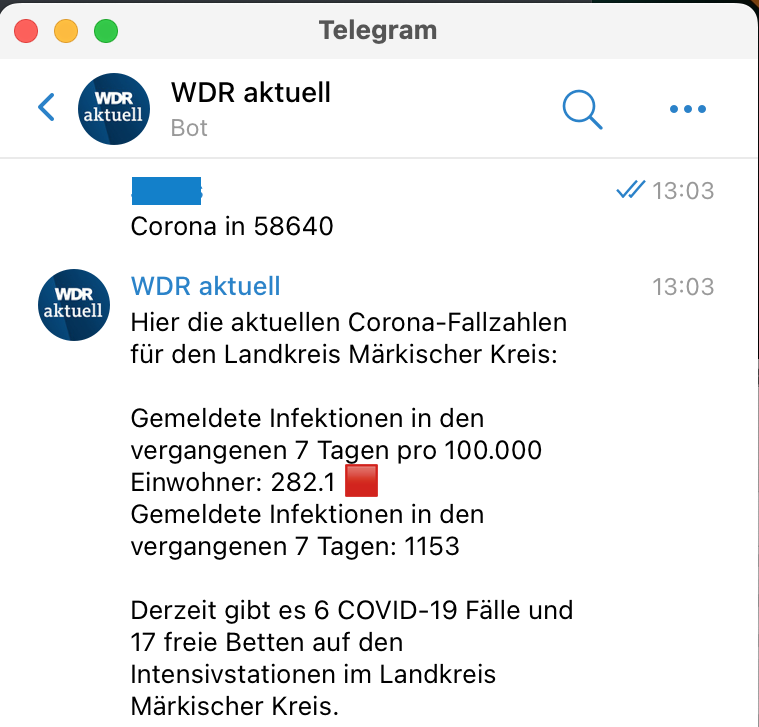
\includegraphics[scale=0.7]{telegram-bot-beispiel}
\caption{Interaktion mit dem Bot von WDR aktuell in Telegram für macOS.}
\end{figure}

\subsubsection{Beziehen von Aktualisierungen von der Telegram API}
\label{sec:telegram-getting-updates}

Laut der technischen Dokumentation der Telegram API \footnote{\url{https://core.telegram.org/bots/api\#getting-updates}} stehen zwei Möglichkeiten zur Verfügung, um Aktualisierungen zu erhalten: \lstinline{long-polling} der API-Methode \lstinline{getUpdates()} oder die Verwendung eines \lstinline{webhooks}. Die beiden Möglichkeiten verwenden unterschiedliche Konzepte und bieten damit verschiedene Vor- und Nachteile. Im Fachbereich der Informatik steht der Begriff \lstinline{polling} für eine dauerhafte wiederkehrende Abfrage von Informationen bei einem Dienst. Diese Technik beansprucht viel CPU-Zeit eines Systems und wird aufgrund des geringen Gegenwerts der meist leer ausgehenden Abfragen als teuer bezeichnet. \lstinline{long-polling} beschreibt eine Technik, bei welcher der Client einer HTTP-Abfrage einen verlängerten Zeitraum bis zum Erhalt der Antwort vom Server akzeptiert, ohne die Abfrage aufgrund einer Zeitüberschreitung abzubrechen. Die Länge des Zeitraums ist variabel. \lstinline{long-polling} bietet damit gegenüber dem klassischen \lstinline{polling} den Vorteil, dass die benötigte Rechenzeit durch die verlängerten Abfragezeiträume stark reduziert wird. Die Software- und Betriebssystementwicklung bietet eine Technik, um die Verwendung von teurem \lstinline{polling} zu umgehen: die Verwendung von \lstinline{interrupts} oder \lstinline{callbacks} (zu deutsch "Rückruf"). Hierbei erhält der Absender der Anfrage eine Rückmeldung, sobald die Antwort vorliegt. Der Vorteil dieser Technik ist, dass nach dem Absenden der Anfrage keine CPU-Zeit seitens des Absenders notwendig ist. Es muss jedoch eine Möglichkeit vorhanden sein, den Absender im Falle einer eingehenden Antwort zum Vorgang zurückzuführen, sodass die weitere Bearbeitung möglich wird. Im Falle der Anbindung der Telegram API übernimmt dies der \lstinline{webhook}. Der \lstinline{webhook} muss (durch die Telegram-API) öffentlich aus dem Internet erreichbar und durch den Verwalter des Bots im Vorhinein durch eine entsprechenden URL definiert worden sein. Wird eine Nachricht an den Bot gesendet, prüft die Telegram-API, intern, ob Definitionen für webhooks vorliegen. Im positiven Fall sendet die Telegram API eine HTTP-Anfrage an die URL des webhooks mit den Details zur eingegangenen Nachricht. Nach Erhalt der Anfrage durch den webhook muss dieser die Daten zur verarbeitenden Software zurückführen und die weitere Bearbeitung auslösen.

\subsubsection{Erstellung eines Bots}

Um ein Programm über die Telegram Bot-API anbinden zu können, muss zuvor ein Bot über Telegram erstellt werden. Hierzu wird der Bot \lstinline{@BotFather} verwendet. Sämtliche Einstellungen zu Bots werden über \lstinline{@BotFather} vorgenommen. Soll ein neuer Bot erstellt werden, werden die benötigten Informationen abgefragt. Nachdem der Anzeigename und der Benutzername festgelegt werden, erhält der Benutzer die Zugangsdaten für die HTTP-API und der Bot ist einsatzbereit. \lstinline{@BotFather} kann jederzeit erneut kontaktiert werden, um weitere Einstellungen vorzunehmen: es können Profilbild und Beschreibung geändert, sowie vordefinierte Kommandos festgelegt werden. Der Zugriff auf die HTTP-API erfolgt über die Basis-URL \lstinline{https://api.telegram.org/bot<token>/METHOD_NAME} \footnote{https://core.telegram.org/bots/api\#making-requests}, wobei \lstinline{<token>} der von \lstinline{@BotFather} erhaltene Zugriffsschlüssel und \lstinline{METHOD_NAME} die API-Methode (beispielsweise \lstinline{getUpdates} oder \lstinline{sendMessage}) ist. Weitere laut API-Dokumentation benötigte Parameter werden als Parameter der HTTP-Anfragen vom Typ \lstinline{GET} oder \lstinline{POST} übermittelt. Die Antwort der API erfolgt in Form eines JSON-Objekts.

\begin{lstlisting}[caption={Beispiel eines Aufrufs der Telegram HTTP-API. Erhalt einer Textnachricht "Hallo Welt".}, label=lst:bsp-telegram-api]
GET https://api.telegram.org/bot123456:ABC-DEF1234ghIkl-zyx57W2v1u123ew11/getUpdates

{
    "ok": true,
    "result": [
        {
            "update_id": 987654321,
            "message": {
                "message_id": 626,
                "from": {
                    "id": 12345678,
                    "is_bot": false,
                    "first_name": "Jonas",
                    "username": "-entfernt-",
                    "language_code": "de"
                },
                "chat": {
                    "id": 12345678,
                    "first_name": "Jonas",
                    "username": "-entfernt-",
                    "type": "private"
                },
                "date": 1662808990,
                "text": "Hallo Welt"
            }
        }
    ]
}
\end{lstlisting}

\section{Graylog Open}

Graylog Open ist ein Softwareprodukt der Firma Graylog, Inc mit dem Hauptsitz in Houston, Texas in den USA. Das Produkt stellt eine kompakte Verwaltungsoberfläche für die Erfassung von Systemprotokollen bereit, welche in einer ElasticSearch Suchmaschine vorgehalten werden. Der Quellcode der Software kann öffentlich eingesehen werden \footnote{\url{https://github.com/Graylog2/graylog2-server}}. Hohe Anforderungen an die (Ausfall-)sicherheit moderner und komplexer IT-Systeme führen zu der Notwendigkeit, die Funktionsfähigkeit der Systeme möglichst allumfassend und automatisiert zu prüfen. Herkömmliche Monitoringsysteme mit einem Fokus auf die Erreichbarkeit oder die Überwachung von vordefinierten Fehlerausgaben erfüllen diese Anforderungen nicht. Fehlerzustände sollen in Echtzeit, möglichst vor und spätestens zum Zeitpunkt einer durch den Anwender spürbaren Einschränkung auffallen. Informationstechnische Systeme in sämtlichen Bereichen sind längst zu komplex geworden, um alle Fehlerquellen im Vorhinein bestimmen und gezielt überwachen zu können. Aus diesem Grund wird ein anderer Ansatz als beim herkömmlichen Monitoring angewendet: die Erfassung der Systemprotokolle der zu überwachenden Systeme. Diese ermöglichen einen umfassenderen Blick auf die aktuellen Ereignisse. Durch die Anwendungsprotokolle können Fehlerzustände eines Webservers beispielsweise bereits nach dem ersten Besuch eines Besuchers einer durch den fehlerhaften Webserver beeinträchtigten Webseite erkannt werden.

\subsection{Erfassung von Systemprotokollen}

Graylog Open ist kompatibel zu einer Vielzahl heutiger Betriebssysteme und Anwendungen. Linuxbasierte Systeme verwenden häufig einen Dienst zur zentralen und systemweiten Erfassung der Anwendungsprotokolle, welcher das in RFC 3164 standardisierte Protokoll \lstinline{syslog} \footnote{\url{https://www.ietf.org/rfc/rfc3164.txt}} verwendet. Dieser schreibt in der Standardkonfiguration vieler aktueller Betriebssysteme auf Basis des Linux Derivats Debian alle Meldungen in Textform in die Datei \lstinline{/var/log/syslog}, bei Systemen auf Basis des Derivats RedHat Enterprise Linux in die Datei \lstinline{/var/log/messages}. Die Position dieser Ausgabedatei auf dem Dateisystem ist für die Verarbeitung der Meldungen in Graylog jedoch nicht wichtig, da die Meldungen nach einer Anpassung der Konfiguration des Dienstes (offiziell wird die Software \lstinline{rsyslog} und \lstinline{syslog-ng} von Graylog unterstützt \footnote{\url{https://docs.graylog.org/docs/syslog}} über das Netzwerk per UDP und optionaler TLS-Verschlüsselung an Graylog übertragen werden. In Graylog muss hierzu die Annahme von Daten über das Netzwerk mit dem syslog-Protokoll aktiviert werden. Mittels einer Input-Konfiguration wird ein Port an der zum überwachenden System nächstgelegenen Netzwerkschnittstelle eröffnet, auf welchem die Software auf eintreffende Meldungen im syslog-Format lauscht.

Auch mit Docker bereitgestellte Microservices können global überwacht werden, ohne die Konfiguration der Container oder sogar die der Anwendungen in einem gestarteten Container einzeln anpassen zu müssen. Hierzu wird nicht das syslog-Protokoll, sondern das von Docker ohnehin unterstützte \footnote{\url{https://docs.docker.com/config/containers/logging/gelf/}} Protokoll GELF verwendet. Es ist ebenfalls eine zentrale Änderung der Konfiguration des Docker-Dienstes notwendig, um fortan die Protokolle aller neu gestarteten Container über das wahlweise UDP- oder TCP-basierte GELF-Protokoll an die Graylog-Instanz zu senden. Die an Graylog übertragenen Daten entsprechen der Ausgabe des \lstinline{docker logs} Kommandos. Um den Empfang von Daten über das GELF-Protokoll seitens Graylog zu ermöglichen, ist es analog zur Einrichtung für das syslog-Protokoll notwendig, mittels einer Input-Konfiguration einen Port auf einer Netzwerkschnittstelle zu reservieren.

Systemprotokolle aus Windows können nicht direkt verarbeitet werden. Es ist der Einsatz einer Middleware wie Winlogbeat notwendig, welche die Protokolle auf dem System erfasst und die Daten über ein Netzwerkprotokoll an Graylog sendet. \footnote{\url{https://docs.graylog.org/docs/windows}}

\subsection{Verarbeitung}

Für die Verarbeitung der erfassten Daten stellt Graylog dem Systemadministrator eine Vielzahl von Möglichkeiten zur Verfügung, welche aufgrund der Fokussierung der Abschlussarbeit auf die Implementierung eines Bots für die Informationsabfrage aus Graylog mittels der angebotenen REST-API nur bezogen auf das Ziel der Abschlussarbeit erläutert werden. Nach der Erfassung der Daten über die konfigurierten Input-Kanäle werden diese in einer Elasticsearch Suchmaschine hinterlegt und nach vom Administrator definierten Filterausdrücken durchsucht. Schließlich sind die erfassten Nachrichten über die Weboberfläche durchsuchbar. Für die Suche wird eine an Apache Lucene (Programmbibliothek für Volltextsuche) angelehnte Syntax verwendet. Der Administrator kann Informationen mittels regulären Ausdrücken aus eingehenden Nachrichten extrahieren und die Graylog-Instanz so auf die zu überwachenden Applikationen anpassen. Beispielsweise kann der HTTP Statuscode eines Eintrags von einem Webserver extrahiert werden:

\begin{figure}[h!]
\centering
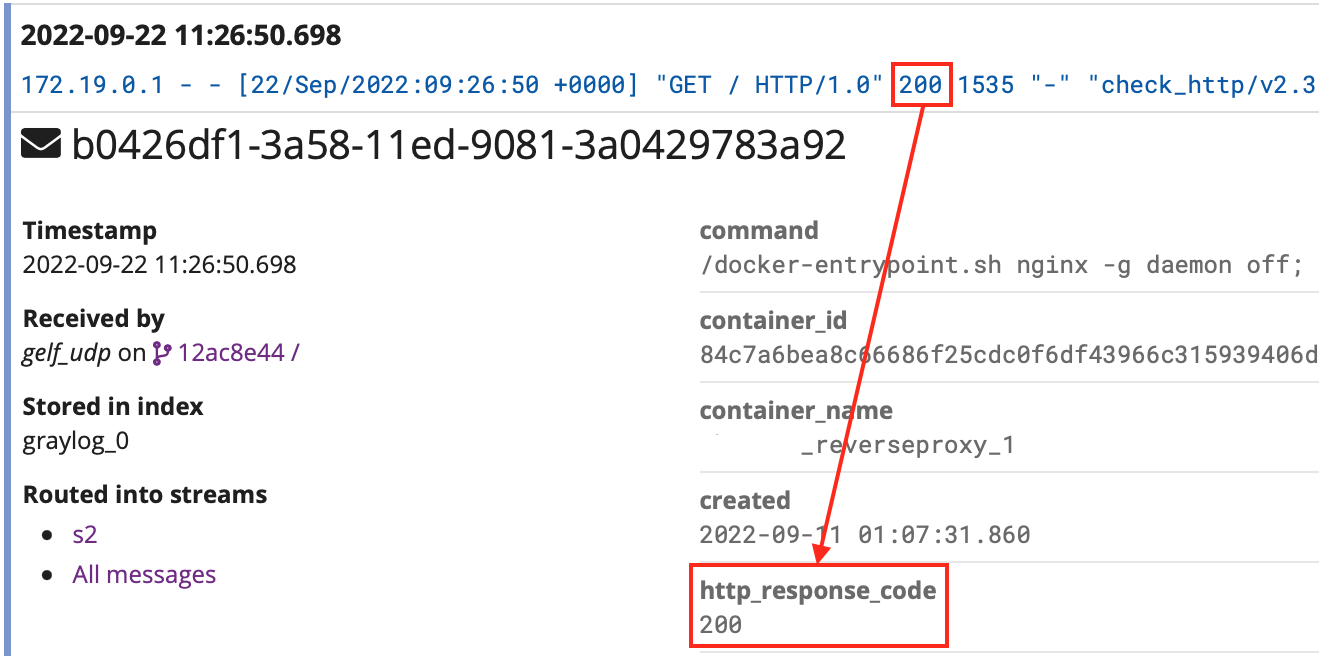
\includegraphics[scale=0.7]{graylog-bsp-msg}
\caption{Extrahieren von Daten aus eingehenden Meldungen in Graylog.}
\end{figure}

\subsection{Zugriff per API}

Graylog stellt eine REST-API zur Verfügung, auf welche sowohl mit der integrierten Webschnittstelle als auch per Fernzugriff zugegriffen werden kann. Die integrierte Webschnittstelle nutzt die API für das Beziehen der Informationen aus der ElasticSearch Suchmaschine. Jede Graylog-Instanz verfügt standardmäßig über eine auf der API-Dokumentationssoftware Swagger basierende Übersicht der verfügbaren Funktionen. Die Oberfläche ermöglicht es zusätzlich, die API-Funktionen aus dem Browser heraus mit selbstgewählten Parametern aufzurufen. Softwareentwickler erhalten so eine Übersicht über die in der installierten Graylog-Version verfügbaren API-Funktionen. Das prüfen von API-Funktionen mit Drittanbieterprogrammen wie curl oder Postman entfällt.

\section{Amazon Web Services}

Der Cloudanbieter AWS ist ein Tochterunternehmen des US-amerikanischen Versandhändlers Amazon. Das Unternehmen bietet seine Dienste vor allem für professionelle Endanwender und Unternehmen an. AWS bietet eine Vielzahl von Diensten, welche "on-demand" (zu deutsch "auf Abruf") verfügbar sind nach dem Prinzip "pay as you go" (zu deutsch "abgerechnet nach Verbrauch") berechnet werden. Zu den bekanntesten Diensten zählen EC2 (elastic compute cloud), welcher virtuelle Maschinen bereitstellt sowie S3 (simple storage service), für das Buchen von Speicherkapazität. AWS gehört neben den allesamt US-amerikanischen Anbietern Microsoft Azure, Google Cloud, Oracle Cloud sowie dem chinesischen Anbieter Alibaba Cloud laut dem Anbieter für Marktforschungsergebnisse Gartner zu den führenden Cloudanbietern weltweit. Derzeit gibt es keinen gleichwertigen Anbieter aus Europa. Die Anbieter IONOS und Strato aus Deutschland sowie OVH aus Frankreich bieten nur einen Bruchteil der Umfänge der Konkurrenten an. Das Projekt GAIA-X verfolgt ein ähnliches Ziel, befindet sich allerdings noch in einem frühen Stadium der Entwicklung.

AWS betreibt zahlreiche Rechenzentren weltweit und stellt einen Großteil der Dienste an allen Standorten zur Verfügung. Zahlreiche Dienste lassen sich über die Webschnittstelle "AWS Konsole" verwalten. Als on-demand Anbieter steht für sämtliche Dienste auch die Bedienung über eine API-Softwareschnittstelle zur Verfügung, sodass Ressourcen bei Bedarf von Programmen selbstständig gebucht und vollständig verwaltet werden können. Die Abrechnung variiert je nach Dienst. Rechenressourcen werden nach Stunden oder Minuten abgerechnet, Speicherressourcen nach Datenmenge und auftragsbasierte Dienste (vgl. \autoref{sec:amazon-transcribe}) nach Auftragskontingenten. AWS bietet zusätzlich ein freies Kontingent an. Die anfallenden Kosten lassen sich im Vorhinein mit dem AWS Pricing Calculator \footnote{\url{https://calculator.aws/}} bestimmen. 

\subsection{Amazon Transcribe}
\label{sec:amazon-transcribe}

Mit dem Dienst Amazon Transcribe können Audiodateien zu Text mittels künstlicher Intelligenz transkribiert werden. Der Dienst unterstützt mehrere Sprachen und Dialekte. Standardmäßig wird ein allgemeines Sprachmodell des Anbieters verwendet. Es ist ebenfalls möglich, ein eigenes Sprachmodell zu trainieren und importieren. Bei der Bedienung über die AWS Konsole muss ein URI zu einer Audiodatei in einem S3-Speicher angegeben werden. Der Dienst hinterlegt den Text in einer Datei ebenfalls in einem S3-Speicher, optional kann dabei der Quellspeicher eingestellt werden. Eine Übersetzung in Echtzeit ist nicht möglich. Das Limit für gleichzeitige Vorgänge pro Benutzer liegt bei 100. Neue Aufträge können so lange nicht eingereicht werden, bis die Anzahl wieder unter dem Limit liegt. Bei einer absehbaren Überschreitung des Limits kann eine Auftragswarteschlange verwendet werden, um die Aufträge zuzuführen. Die Abrechnung erfolgt außerhalb des freien Kontingents nach Zeitkontingenten und beginnt bei 0,024 USD pro angefangene Minute.

\subsection{Amazon Polly}
Polly ist ein TTS-Dienst (Text-To-Speech, zu deutsch "Text zu Sprache") und bildet das Gegenstück zu Amazon Transcribe. Der Dienst unterstützt ebenfalls verschiedene Sprachen und Dialekte. Je nach Sprache können verschiedene Modelle verwendet werden, welche verschiedene Persönlichkeiten und Geschlechter darstellen. Dabei wird zwischen den Typen "Standard" und "Neural" unterschieden. "Neural"-Modelle erzeugen eine gegenüber des Typs "Standard" optimierte Ausgabe, welche der menschlichen Aussprache so ähnlich wie möglich kommen soll. Die Abrechnung erfolgt außerhalb des freien Kontingents nach Zeichenkontingenten und beginnt bei 4 USD für eine Million Zeichen. Der Typ "Neural" kostet bei gleicher Verwendung etwa das Vierfache. 

\chapter{Planung}
\label{cha:planung}

In diesem Kapitel werden Anforderungen an die Software und die Systemumgebung definiert sowie verwendete organisatorische Konzepte erläutert.

\section{Anforderungen}

Die Software soll auf den nicht-interaktiven Betrieb als Dienst auf unix-artigen Betriebssystemen ausgelegt werden. Dies hat u.\,a. Auswirkungen auf die geplanten Benutzerschnittstellen. Das Programm soll zur Laufzeit keine Konsoleneingaben verlangen, da diese nur bei einem interaktiven Betrieb, z.B. in der Shell, vorgenommen werden können. Stattdessen soll mit dem Anwender vollständig über den Telegram-Messenger interagiert werden und administrative Einstellungen sollen über Konfigurationsdateien vorgenommen werden können. 

Zur Anwendung von geänderten Einstellungen ist unter Umständen ein Neustart der Software notwendig. Die Software sollte daher zustandslos arbeiten, um einen möglichen Verlust von eingegangenen und noch nicht verarbeiteten Daten zu verhindern. Weiterhin sollte die durch einen Neustart verursachte Ausfallzeit so gering wie möglich gehalten werden. 

Die Software soll Ereignismeldungen über die Standardausgabe sowie über eine textbasierte Protokolldatei ausgeben, um Fehleranalysen zu vereinfachen. Es soll möglich sein, den Bot von mehreren Geräten gleichzeitig zu kontaktieren. Der Bot muss die Autorisierung von Benutzern prüfen, damit unerwünschter Datenabfluss verhindert wird.

\subsection{Systemumgebung}
Für den Betrieb der Software ist eine vorinstallierte Python 3 Umgebung notwendig. Zum Zeitpunkt der Entwicklung wurde die Version 3.9 verwendet. Die benötigten Bibliotheken sollen über den Paketmanager Pip bezogen und aktuell gehalten werden können. Auch wenn die Software auf den Betrieb als Dienst ausgelegt wird, soll eine interaktive Verwendung mit unix-artigen Betriebssystemen möglich sein. Außerdem ist eine Internetverbindung notwendig, um die Server der HTTP-APIs von Telegram und AWS zu erreichen. Graylog Open muss bereits installiert und an die zu überwachenden Systeme angeschlossen sein. Die Systemanforderungen entsprechen denen des verwendeten Betriebssystems. Da sämtliche Verbindungen zu externen Systemen via HTTP(S)-Verbindungen hergestellt werden, gibt es keine weiteren Anforderungen für den Betrieb der Software. Für eine Minimalkonfiguration kann die Software in vollem Funktionsumfang bereits beim Betrieb in einer Softwareentwicklungsumgebung, z.B. auf einem Notebook verwendet werden. Für den späteren Produktivbetrieb eignet sich ein System, welches günstig dauerhaft betrieben werden kann, beispielsweise eine AWS EC2-Instanz.

\section{Programmablauf}

\subsection{Selbsttest}
\label{sec:grundsaetzlicher-aufbau}

Nach dem Start der Software muss geprüft werden, ob ein einwandfreier Betrieb möglich ist. Dazu ist es notwendig, die Erreichbarkeit und Funktion sämtlicher Dienste mittels geeigneter API-Abfragen zu prüfen. Nachdem die Vorbereitungen abgeschlossen sind, kann in den Regelbetrieb übergegangen werden, in welchem sich das Programm bis zum Programmende befindet. 

\subsection{Regelbetrieb}

Im Regelbetrieb reagiert die Software in Echtzeit auf eingehende Nachrichten vom Anwender. 
Um den Betrieb der Software auch mit nicht-öffentlichen IP-Adressen (beispielsweise in einem Heimnetzwerk hinter einem NAT-Router) oder einer Firewall, welche den Zugriff auf Geräte im internen Netzwerk aus dem Internet verbietet, zu ermöglichen, soll das Verfahren des Long-polling für den Abruf von Informationen von der Telegram API verwendet werden (vgl. \hyperref[sec:telegram-getting-updates]{erstes Unterkapitel von Abschnitt 2.2.1}). Somit werden lediglich Verbindungen aus dem internen Netzwerk ins Internet aufgebaut. Eventuelle NAT-Router oder Firewalls hinterlegen den Verbindungsaufbau in internen Datenstrukturen wie NAT-Tabellen und lassen Antworten aus dem Internet zu.

Der geplante Ablauf des Regelbetriebs ist im Sequenzdiagramm in \autoref{fig:dia-seq} abgebildet.

\subsection{Spracherkennung}

Bei der Ausarbeitung eines Konzepts für die Funktionsweise der Spracherkennung müssen einige funktionale und nicht-funktionale Eigenschaften beachtet werden. Die Entscheidung wird u.\,a. beeinflusst durch Aspekte der ... 

\begin{itemize}
\item Erweiterbarkeit: es soll einfach und insbesondere ohne ein notwendiges Training von Sprachmodellen möglich sein, neue Systeme und Abfragen zu definieren.
\item Fehlertoleranz: gesprochene Sprache enthält Umgangssprache und verändert sich durch grammatikalische Eigenschaften je nach Satzbau leicht in der Aussprache. Die Erkennung muss trotz dieser Veränderungen zuverlässig funktionieren.
\item Rechenkapazität: die Geschwindigkeit (Wartezeit während des Vorgangs) der Spracherkennung sollte nicht von begrenzten Rechenressourcen oder der Länge der zu übersetzenden Nachricht abhängen.
\item finanziellen Kosten: diese sollten möglichst gering gehalten werden.
\item Plattformunabhängigkeit: die Software und ggf. trainierte Modelle sollten wie die gewählte Programmiersprache Python plattformunabhängig und portabel sein.
\item Nachvollziehbarkeit: während der Entwicklung und bei der Definition neuer Begriffe sollten auftretende Fehler einfach erkenn- und behebbar sein.
\item Sprache: das System soll Sätze verstehen, welche Begriffe aus mehreren Sprachen (Deutsch und Englisch) beinhalten.
\end{itemize}

Es bestehen verschiedene Möglichkeiten, Sprache zu Text zu transkribieren und den Inhalt im Anschluss zu analysieren, um das Anliegen des Anwenders zu erkennen und eine passende Anfrage für die Suchmaschine in Graylog zu bilden. Für die Transkription ist es notwendig, künstliche Intelligenz einzusetzen. Diese kann lokal oder entfernt ausgeführt werden. Die entfernte Ausführung bietet Vorteile bezüglich der Plattformunabhängigkeit und der (von den lokalen Ressourcen unabhängigen) Geschwindigkeit. Es stehen verschiedene Online-Dienste für die Transkription zur Verfügung, darunter Watson Speech to Text von IBM, Amazon Transcribe von AWS und Speech-To-Text vom Anbieter Google Cloud. 

\subsubsection{Vergleich diverser Transkriptionsdienste}
\label{sec:vergleich-transkrip}

Die Umwandlungsgenauigkeit der genannten Dienste soll mit einem Testset bestehend aus umzuwandelnden Audiodateien mit möglichen Sprachanfragen geprüft werden. Dazu wurden zehn Sprachnachrichten über die Telegram App für iOS auf einem iPhone aufgenommen. Im Anschluss wurden die Audiodaten von der Telegram API extrahiert, sodass diese im OGG-Format vorlagen. Die drei Dienste bevorzugen jeweils andere Audioformate, daher wurden die Dateien aus dem OGG-Format (für das Produkt von Google Cloud) in das MP3- (für das Produkt von AWS) und das FLAC-Format (für das Produkt von IBM) umgewandelt. Schließlich wurden jeweils zehn Audiodateien über eine Webkonsole, welche von allen Anbietern angeboten wurde\footnote{\url{https://eu-central-1.console.aws.amazon.com/transcribe/home?region=eu-central-1\#createJob}, \url{https://speech-to-text-demo.ng.bluemix.net}, \url{https://cloud.google.com/speech-to-text}}, an den Dienst übermittelt. Die Webkonsolen verwendeten jeweils die APIs, welche ebenfalls für den programmgesteuerten Zugriff verwendet werden. Die Ergebnisse werden in der \autoref{tab:erg-transkript} abgebildet.

\begin{figure}[h!]
\centering
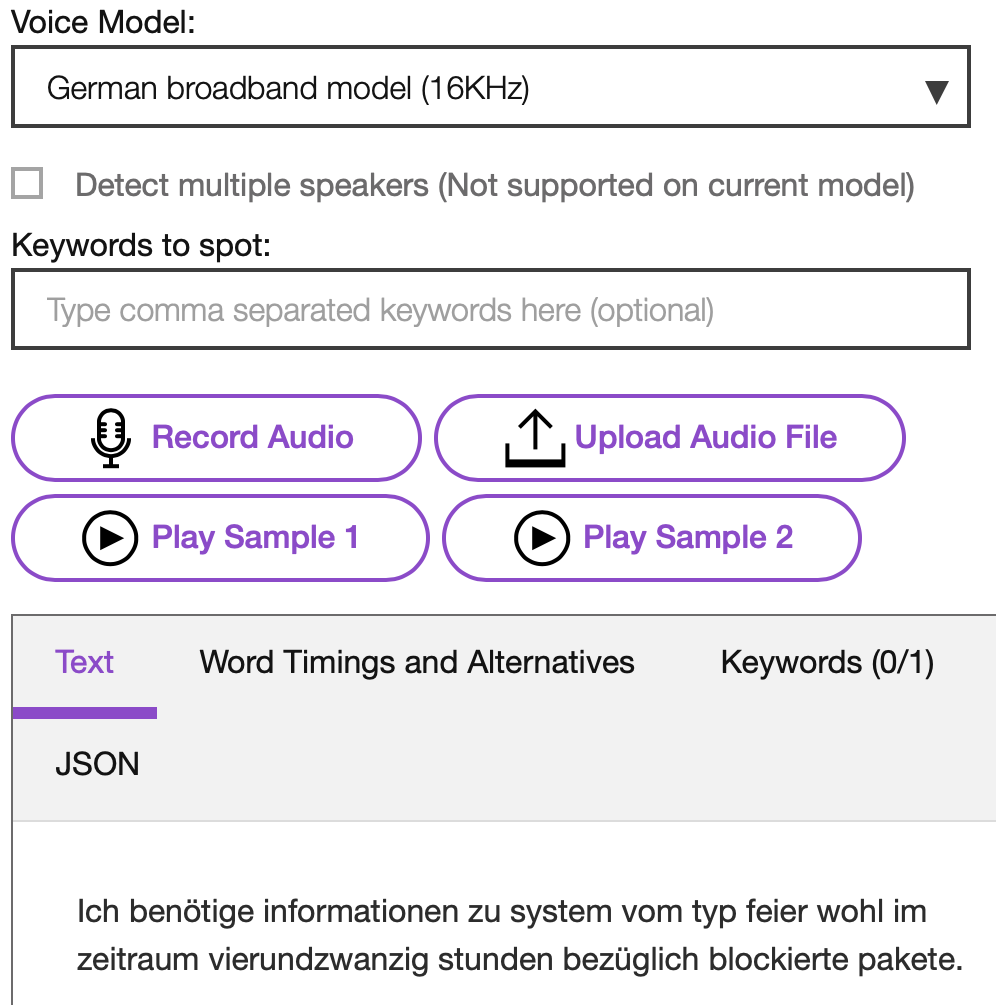
\includegraphics[scale=0.5]{feier-wohl}
\caption{Eingabemaske von IBM Watson Speech to Text nach Bearbeitung von Testset06 mit einer unzutreffenden Ausgabe.}
\label{fig:feier-wohl}
\end{figure}

Die Audionachrichten beinhalten folgende gesprochene Texte:
\begin{itemize}
\item \textit{Testset01}: "Typ Webserver Eigenschaft Fehler Zeitraum 24 Stunden"
\item \textit{Testset02}: "Typ Webserver bezüglich Erreichbarkeit Zeitraum 24 Stunden"
\item \textit{Testset03}: "Typ Webserver bezüglich Besucherzugriffe Zeitraum 24 Stunden"
\item \textit{Testset04}: "Typ Webserver bezüglich Besucherzugriffe Zeitraum 24 Stunden"
\item \textit{Testset05}: "Ich benötige Informationen zu Systemen vom Typ Firewall im Zeitraum 24 Stunden bezüglich blockierte Pakete"
\item \textit{Testset06}: "Typ eins bezüglich drei Zeitraum ein Tag"
\item \textit{Testset07}: "Typ eins bezüglich drei Zeitraum ein Tag"
\item \textit{Testset08}: "Typ Webserver Zeitraum 24 Stunden bezüglich Erreichbarkeit"
\item \textit{Testset09}: "Typ Webserver Zeitraum 24 Stunden bezüglich Erreichbarkeit"
\item \textit{Testset10}: "Typ Mailserver bezüglich empfangene Mails Zeitraum ein Jahr"
\end{itemize}

\begin{table}[hb!]
\centering
\begin{tabular}{c|c|c|c}
Testset 		& AWS	& Google		& IBM \\
\hline
01			& -		& +			& + \\
02			& +		& +			& - \\
03			& +		& +			& + \\
04			& -		& -			& - \\
05			& +		& +			& - \\
06			& +		& +			& - \\
07			& +		& +			& - \\
08			& +		& +			& - \\
09			& +		& -			& - \\
10			& +		& +			& - \\
\hline
Summe Fehler	& 2		& 2			& 8
\end{tabular}
\caption{Ergebnisse der Transkriptionsaufträge.}
\label{tab:erg-transkript}
\end{table}

Die Transkriptionsdienste von AWS und Google Cloud konnten durch eine geringe Fehlerquote gegenüber dem Produkt vom IBM überzeugen. Aufgrund von bereits existierenden persönlichen Erfahrungen in der Verwendung von AWS wird Amazon Transcribe als Transkriptionsdienst verwendet.

\subsubsection{Syntax}
\label{sec:syntax}

Liegt die eingegangene Nachricht als Text vor, müssen die Inhalte analysiert werden. Der Aufbau der Nachricht muss einem festen Muster folgen, welches durch eine Prozedur analysiert werden kann. Hierzu eignet sich die Verwendung von Schlüsselwörtern. Diese bieten den Vorteil, dass keine Analyse der Grammatik notwendig ist. Die Verwendung von künstlicher Intelligenz bietet hierbei keine Vorteile. Das KI-Modell müsste für neue Begriffsdefinitionen, Grammatik (Satzbau) sowie Umgangssprache trainiert werden. Dies ist bei der geplanten Anwendung des Programms nicht durchführbar, da der Aufwand für das Hinzufügen neuer Suchbegriffe möglichst gering gehalten werden soll. Weiterhin bietet ein Algorithmus für die Analyse einer Nachricht mit statischem Aufbau den Vorteil der besseren Nachvollziehbarkeit des ermittelten Ergebnisses.

Es wird ein Aufbau aus Produktkategorie, Eigenschaft und Zeitraum gewählt. Die Produktkategorie entspricht der abzufragenden Gerätegruppe, beispielsweise 'Webserver'. Für jede Produktkategorie können Eigenschaften definiert werden, für die Abfrage von Ereignissen mit einem Statuscode \lstinline{4xx} oder \lstinline{5xx} der Gruppe 'Webserver' beispielsweise 'Fehlermeldungen'. Ein weiteres Schlüsselwort führt zu den Informationen für den abzufragenden Zeitraum, welcher relativ angegeben wird ('letzte fünf Tage', 'letzte Woche', 'letzte 20 Minuten'). Schließlich muss die Erkennung von Zahlwörtern zuverlässig funktionieren.

\subsubsection{Verknüpfung geeigneter Suchbegriffe}

Die Erweiterung der Software soll einfach möglich sein. Produktgruppen sollten darüber hinaus dynamisch erweiterbar sein: Wird eine Abfrage für die Produktkategorie 'Webserver' getätigt, sollen alle derzeit an Graylog angeschlossenen Webserver in die Suche einbezogen werden. 

Die Software ist für die Bedienung durch Systemadministratoren vorgesehen. Daher soll für die Konfiguration der Abfragen eine Textdatei verwendet werden. Diese ermöglicht eine schnelle Anpassung der Konfiguration und bietet gleichzeitig einen Überblick über bestehende Suchbegriffe. Für die einfache Verwendung mit einer Python-Bibliothek stehen mehrere Dateiformate zur Verfügung, darunter JSON, INI, TOML, YAML und XML. Das YAML- und XML-Format ist für die Verwaltung über einen Texteditor ohne Syntaxhervorhebung und Funktionen wie automatischem Einrücken nicht geeignet. 

Das TOML-Format vereint die Vorteile der einfachen Lesbarkeit des INI-Formats mit der Fehlerunanfälligkeit bei der Verarbeitung durch Maschinen des JSON-Formats. TOML entspricht weitestgehend der INI-Syntax mit dem Unterschied, dass Anführungszeichen verwendet werden können, um Anfang und Ende von Werten zu markieren. Die Hierarchie innerhalb einer TOML-Datei stimmt mit dem im \hyperref[sec:syntax]{vorherigen Unterkapitel "Syntax"} gebildeten Aufbau überein. Sektionen werden mit eckigen Klammern markiert und entsprechen den Produktkategorien. Sie beinhalten Name-Wert-Paare, welche durch ein Gleichheitszeichen getrennt werden. Ein Name darf in einer Sektion nur jeweils einmal vorkommen, eine Sektion darf in einer Datei nur jeweils einmal vorkommen. Bestehen Namen aus mehreren Wörtern, können diese mit Anführungszeichen zusammengefasst werden. Namen entsprechen den oben definierten Eigenschaften von Produktkategorien. Werte entsprechen grundsätzlich einem festgelegten Datentyp. Strings (Zeichenketten) werden in Anführungszeichen geschrieben. Die Werte einer TOML-Datei entsprechen den mit Eigenschaften verknüpften Suchbegriffen. Zusätzlich ist es möglich, einzeilige Kommentare mit \lstinline{#} einzuleiten.

\begin{lstlisting}[caption={Beispiel der TOML-Syntax.}, label=toml-syntax, xleftmargin=6mm]
# Dies ist ein Kommentar
[Sektion]
Name = "Wert"

[Webserver]
Fehler = http_response_code:[400 TO 599] 
\end{lstlisting}

\begin{figure}[h!]
\centering
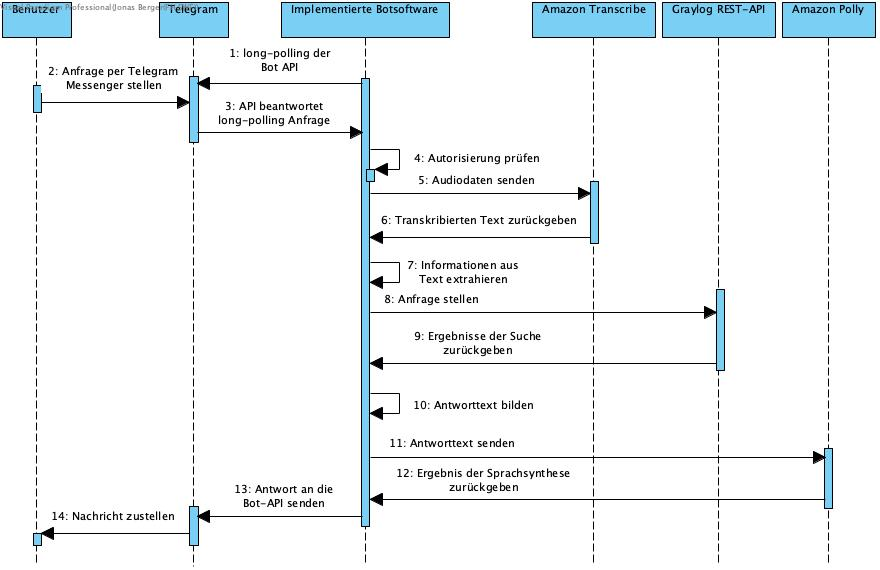
\includegraphics[scale=0.8,angle=90,origin=c]{dia-seq}
\caption{Sequenzdiagramm für Regelbetrieb.}
\label{fig:dia-seq}
\end{figure}

\chapter{Implementierung}
\label{cha:implementierung}

\section{Auswahl der Programmiersprache}

Die Software soll in der Skriptsprache Python entwickelt werden. Für die Entscheidung sprechen mehrere Vorteile: die Plattformunabhängigkeit wird durch die Verfügbarkeit von Interpretern sowohl für unix-artige Betriebssysteme als auch Windows ermöglicht. Die Software liegt jederzeit im Quellcode vor und kann so einfach gewartet und erweitert werden. Des weiteren existiert aufgrund der hohen Popularität\footnote{\url{https://www.tiobe.com/tiobe-index/python/}} eine reichhaltige Auswahl an Bibliotheken und Onlinedokumentationen, welche die Entwicklung der Software vereinfachen. 

\section{Struktur}

Um eine modulare Implementierung der Software zu ermöglichen und darüber hinaus den Quellcode getrennt von nicht für die Öffentlichkeit bestimmten Daten (beispielsweise Anmeldedaten für APIs) bereitstellen zu können, ist es notwendig, die Softwareentwicklungsumgebung entsprechend zu gestalten. Die Unterteilung der für den Betrieb notwendigen Dateien inkl. des Quellcodes wird in den folgenden beiden Unterkapiteln beschrieben. Um die Lesbarkeit und Erweiterbarkeit zu verbessern, wurden die im Python Enhancement Proposal (PEP) Nr. 8\footnote{\url{https://peps.python.org/pep-0008/}} vorgeschlagenen Formatierungsrichtlinien umgesetzt. Sämtliche Module und Funktionen enthalten nach der Definition einen mehrzeiligen Kommentar mit einer Docstring-Dokumentationen gemäß PEP 257\footnote{\url{https://peps.python.org/pep-0257/}} im Quellcode.

\subsection{Dateisystem}

Nachfolgend wird die Struktur der in \autoref{fig:dateisystem} dargestellten Ordner und Dateien erläutert.

\begin{figure}[h!]
\centering
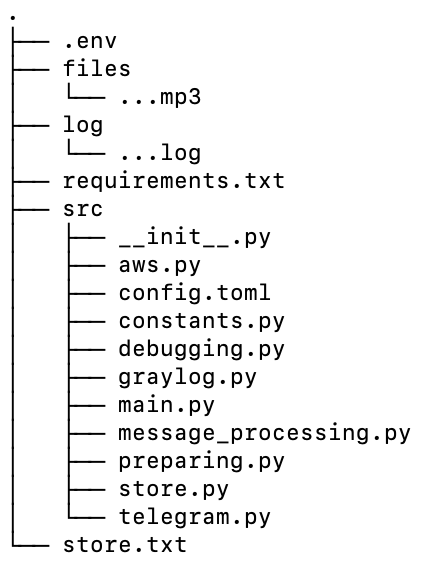
\includegraphics[scale=0.75]{dateisystem}
\caption{Gekürzte Ausgabe der für den Betrieb notwendigen Ordner und Dateien im Basisverzeichnis.}
\label{fig:dateisystem}
\end{figure}

Von oben nach unten: 

\begin{itemize}
\item '.env' beinhaltet sensible Zugangsdaten für die verschiedenen Dienste und wird nicht in das öffentliche GitHub-Repository hochgeladen. 
\item 'files' dient als Zwischenspeicher für anfallende Audiodateien, welche aus den eingehenden Sprachnachrichten extrahiert wurden oder per Sprachsynthese erzeugt wurden. 
\item 'log' enthält die textbasierten Protokolle der Software. Zu jedem Start der Software wird eine neue Datei mit dem aktuellen Datum erzeugt. Die Inhalte der Dateien entsprechen der Konsolenausgabe mit der Ausnahme, dass sensible Daten nur in der Konsolenausgabe ausgegeben werden. 
\item requirements.txt dient als Informationsquelle für den Paketmanager Pip, mit welchem die Abhängigkeiten aus dem Python Package Index installiert werden können. Die Datei beinhaltet Namen und Versionsnummern von externen Softwaremodulen. 
\item 'src' beinhaltet Dateien mit dem Quellcode. 
\item '\_\_init\_\_.py' ist notwendig für die Moduldefinitionen in Python und hat keinen Inhalt 
\item 'store.txt' wird für die Persistierung des Werts für den Parameter 'update\_id' der Telegram Bot API verwendet.\cite[S. 337]{python}.

Weitere Dateien im Quellcode-Verzeichnis entsprechen den Modulen und werden im folgenden \autoref{sec:module} detaillierter erläutert. 

\end{itemize}

\subsection{Module}
\label{sec:module}

Der Quellcode wurde in mehrere Module aufgeteilt:

\begin{itemize}
\item \lstinline{main}: enthält die Hauptfunktion des Programms und startet die Vorbereitung und den Übergang in den Regelbetrieb.
\item \lstinline{debugging}: enthält die für die Fehlersuche notwendigen Funktionen. Siehe \autoref{sec:protokollierung}.
\item \lstinline{preparing}: enthält die für den Startvorgang notwendigen Funktionen, welche nicht Teil eines anderen Moduls sind. Siehe \autoref{sec:startvorgang}.
\item \lstinline{telegram}: enthält Funktionen für den Zugriff auf die Telegram-API. Die HTTP-Abfragen werden mit der Programmbibliothek \lstinline{requests}\footnote{\url{https://pypi.org/project/requests/}} durchgeführt. Weiterhin sind Funktionen für die Bearbeitung der Antworten der API enthalten. Die Authentifizierung an der API erfolgt über nur dem Entwickler bekannte Zugriffsschlüssel, welche vom Telegram-Bot \lstinline{@BotFather} ausgestellt werden.
\item \lstinline{aws}: enthält Funktionen für den Zugriff auf AWS. Für die Kommunikation mit der API wird das SDK für die Programmiersprache Python des AWS-Teams \lstinline{boto3} verwendet. Die Verwendung der Python SDK für AWS 'boto3' gegenüber einer 'low-level' Implementierung der HTTP-Abfragen mit der Programmbibliothek \lstinline{requests} bringt mehrere Vorteile, beispielsweise in der Sitzungsverwaltung. Weiterhin bietet die boto3-Bibliothek die Möglichkeit, für ausgesuchte Dienste einen mehr objektorientierten und von API-Funktionen abstrahierten Zugriff zu verwenden\footnote{\url{https://boto3.amazonaws.com/v1/documentation/api/latest/guide/resources.html}}.
\item \lstinline{constants}: beinhaltet Konstanten, mit welchen der Ablauf des Programms gesteuert werden kann (beispielsweise können detaillierte Meldungen zum Programmablauf aktiviert oder bestimmte Telegram-Benutzer für den Zugriff auf den Bot autorisiert werden). Des Weiteren sind Variablen als Platzhalter Teil des Moduls, welche zur Laufzeit mit Objektdefinitionen der boto3-Bibliothek überschrieben werden. Dies ermöglicht einen durchgehenden Zugriff auf die AWS-API ohne wiederkehrende Authentifizierungen.
\item \lstinline{graylog}: beinhaltet Funktionen für den Zugriff auf die Graylog API. Der Zugriff erfolgt ähnlich wie beim Modul \lstinline{telegram} mit der Programmbibliothek \lstinline{requests}. Aus Sicherheitsgründen werden verschiedene Zugangsschlüssel für die Autorisierung und Authentifizierung verwendet\footnote{\url{https://docs.graylog.org/docs/rest-api}}. Der 'access token' (dt. 'Zugriffsschlüssel') entspricht den Anmeldedaten an der Graylog Webschnittstelle und ermöglicht einen dauerhaften Zugriff. Mit dem 'access token' können zeitlich befristete 'session tokens' (dt. 'Sitzungsschlüssel') generiert werden. Die Software erkennt anhand der von der API zurückgegebenen Fehlermeldung automatisch, wenn ein nicht gültiger 'session token' verwendet wurde, und beantragt in diesem Fall einen neuen.
\item \lstinline{message_processing}: enthält interne Funktionen, welche für die Verarbeitung der erhaltenen Nachrichtentexte vorgesehen sind. 
\item \lstinline{store}: enthält Funktionen, welche für die Persistierung von Informationen notwendig sind. Die Telegram-API verwendet einen Zähler, welcher für jede Aktualisierung um einen Schritt inkrementiert wird. Ruft der Client Aktualisierungen von der API ab, erhält er den derzeitigen Stand als Wert der Variable 'update\_id' (vgl. \autoref{lst:bsp-telegram-api}). Bei weiteren Anfragen an die API gibt der Client die Variable 'update\_id' an, um nur Aktualisierungen zu erhalten, die seit der letzten Abfrage eingetroffen sind (und daher einen höheren Wert der Variable 'update\_id' haben). Die Variable 'update\_id' wird nach jeder Abfrage in die Textdatei store.txt auf das lokale Dateisystem geschrieben.
\end{itemize}

\section{Protokollierung}
\label{sec:protokollierung}

Für die Protokollierung wurde ein bereits vorhandenes, vom Autor dieser Arbeit entwickeltes Programmmodul erweitert, das Modul 'debugging' des GitHub-Repositorys 'Jomibe/wireguard-config-generator'\footnote{\url{https://github.com/Jomibe/wireguard-config-generator/blob/main/src/debugging.py}}. Das Repository enthält den Quellcode sowie die Dokumentation eines Softwareprojekts, welches im Rahmen des Moduls 'Projekt' im Sommersemester 2022 an der Fachhochschule Südwestfalen implementiert wurde. Es wurde eine Software entwickelt, mit welcher die Konfigurationsdateien eines WireGuard-VPN-Servers verwaltet werden können. Das Programm ermöglicht es unter anderem, die existierenden Konfigurationsdateien auf Syntax- und semantische Fehler zu prüfen und Konfigurationen für weitere VPN-Clients inkl. der Bestimmung von geeigneten Netzwerkkonfigurationen hinzuzufügen. Das Modul 'debugging' enthält Funktionen, welche für die Fehlersuche während der Laufzeit verwendet werden. In dem Modul wird die Funktion \lstinline{console()} implementiert, um die Ausgabe von Statusmeldungen auf der Konsole zentral zu koordinieren. 

Alle Statusmeldungen werden in einer Textdatei hinterlegt, deren Pfad in der Datei 'config.py' konfiguriert wird. Ist der \lstinline{DEBUG}-Modus aktiv, erscheinen alle Meldungen zusätzlich auf der Konsole. Ist die Fehlermeldung mit dem Parameter \lstinline{secret} gekennzeichnet, erfolgt keine Protokollierung in der Textdatei. Werden Meldungen auf der Konsole ausgegeben, werden diese gemäß dem Schweregrad farblich markiert. Dazu wird das Modul 'colorama'\footnote{\url{https://pypi.org/project/colorama/}} verwendet.

Bei der Formulierung der Fehlermeldungen wurden einige Anforderungen beachtet \cite[S. 495]{ux}: 

\begin{itemize}
\item Details zu fehlenden Informationen und Hinweise, wie diese Informationen übermittelt werden können. In diesem Anwendungsfall werden beispielsweise die Schlüsselwörter für Produktkategorien, Eigenschaften und Zeiträume genannt, wenn Informationen dazu fehlen.
\item Vermeidung von technischen Ausdrücken in den Fehlermeldungen.
\item Fehlermeldungen müssen den Benutzer möglichst schnell auf die Fehlerursache hinweisen und dürfen nicht vorwurfsvoll formuliert sein.
\end{itemize}

Im Anhang befinden sich zwei Listings mit den Konsolenausgaben des Programms beim Start (\autoref{log-start}) und beim Verarbeiten einer eingegangenen Nachricht (\autoref{log-msg}).

\section{Startvorgang}
\label{sec:startvorgang}

Das Modul \lstinline{main} enthält die Methode \lstinline{main()}, welche den Startpunkt des Programms darstellt. In der Vorbereitungsphase (vgl. \autoref{sec:grundsaetzlicher-aufbau}) wird zuerst die Programmbibliothek \lstinline{colorama} initialisiert. Dies ist notwendig, um die Steuerung der Farbausgabe auf der Konsole an das zur Laufzeit verwendete Betriebssystem anzupassen\footnote{\url{https://github.com/tartley/colorama\#initialisation}}. Nach der Initialisierung wird die Funktion \lstinline{prepare()} aus dem Modul \lstinline{preparing} aufgerufen. Diese Funktion stellt einen sogenannten 'hook' dar, welcher sämtliche Prüfungen vor Beginn des Regelbetriebs beinhaltet. Wird eine Prüfung nicht erfolgreich abgeschlossen, gibt \lstinline{prepare()} den Wert \lstinline{False} zurück und der Programmablauf wird nach Ausgabe einer detaillierten Fehlermeldung abgebrochen. Falls kein Fehlerstatus zurückgegeben wird, wird zum Regelbetrieb übergegangen. Dieser besteht aus einer Endlosschleife, in welcher die Funktion \lstinline{check_updates()} des Moduls \lstinline{telegram} aufgerufen wird.

\section{Regelbetrieb}

Im Regelbetrieb wird die Funktion \lstinline{getUpdates} der Telegram-API mittels 'long-polling' aufgerufen. Der Wert für den Ablauf der HTTP-Anfrage beträgt standardmäßig 30 Sekunden und kann mittels des Parameters \lstinline{TELEGRAM_LONG_POLL_TIMEOUT} verändert werden.

Eingehende Nachrichten werden in Echtzeit erkannt und weiterverarbeitet. Falls mehrere Nachrichten vorliegen (dies kommt vor, wenn die Software für längere Zeit nicht mit der Telegram-API verbunden war und in der Zwischenzeit mehrere Nachrichten an den Bot gesendet wurden), wird jeweils nur eine Nachricht verarbeitet, da die Variable 'update\_id' nur um jeweils einen Schritt (statt um die Anzahl der neuen Nachrichten) inkrementiert wird. Zuerst wird anhand der Chat ID (vgl. \autoref{lst:bsp-telegram-api}, Zeile 18) ermittelt, ob der Benutzer durch den Administrator für die Verwendung des Bots freigegeben wurde. Hierzu wird der Wert mit der Liste \lstinline{constants.AUTHORIZED_CHAT_IDS} verglichen. Bei positivem Ergebnis erfolgt die Verarbeitung der Nachrichteninhalte: anhand des Aufbaus des JSON-Objekts wird ermittelt, ob es sich um eine Text- oder Sprachnachricht handelt. Der Text einer Nachricht wird direkt durch die Funktion \lstinline{message_processing.process_text_message} verarbeitet. Handelt es sich um eine Sprachnachricht, wird zuerst die Audiodatei von der Telegram Bot-API bezogen und auf dem lokalen Dateisystem abgelegt. Danach erfolgt der Transkriptionsprozess in einer weiteren Funktion, welche den ermittelten Text in einer Zeichenkette zurückgibt. Schließlich wird der Text ebenfalls durch die Funktion \lstinline{message_processing.process_text_message} verarbeitet.

\subsection{Optimierung der Antwortzeit}

Die Bedienung eines Systems mittels Sprache erfordert eine umfangreichere Benutzerführung als die Bedienung eines textbasierten Systems über einen Bildschirm und eine Tastatur. Beim Aufruf einer Webseite in langsamen Netzwerken bietet der Bildschirm durch die Anzeige des Webbrowsers mit diversen Statuselementen eine dauerhafte Möglichkeit für den Benutzer zu prüfen, ob die gewünschte Anfrage eingegangen ist und verarbeitet wird. Eine nur auf Sprache basierende Bedienung bietet keine äquivalente Möglichkeit, dem Benutzer eine Statusübersicht bis zum Abschluss der Anfrage zur Verfügung zu stellen. Um Missverständnisse vorzubeugen und die Bedienung komfortabel zu gestalten, muss das System eine Rückmeldung innerhalb eines durch den Menschen als nicht zu lang empfundenen Zeitraums zurückgeben. Dazu sollte die Zeit ohne sichtbare Veränderung eine Dauer von 10 Sekunden nicht überschreiten \cite[Kapitel 5.5]{response-time}\footnote{Auszug aus dem Buch: \url{https://www.nngroup.com/articles/response-times-3-important-limits/}}. 

Bei der Entwicklung fiel auf, dass die Dauer zwischen Absenden der Sprachnachricht und Erhalt einer Antwort mit den Ergebnissen bis zu 30 Sekunden betrug. Diese Antwortzeit entspricht nicht dem oben genannten Richtwert von 10 Sekunden. Eine Analyse des Programmablaufs ergab, dass die Transkription und die Sprachsynthese (der Text-To-Speech Prozess) einen Großteil der benötigten Antwortzeit verursachten. Beide Prozesse wurden optimiert, die Optimierungen werden in den beiden folgenden Abschnitten beschrieben.

\subsubsection{Transkription}
\label{sec:optimierung-transk}

Ursprünglich wurde die boto3-Bibliothek für die Interaktion mit Amazon Transcribe verwendet. Mit der boto3-Bibliothek ist eine Verarbeitung in Echtzeit nicht möglich. Die Audiodatei muss zuerst in einen S3-Speicher hochgeladen werden. Eine Möglichkeit für die direkte Zuführung der Datei besteht nicht. Im Anschluss muss ein Auftrag in Amazon Transcribe über das \lstinline{client}-Objekt in \lstinline{constants.aws_transcribe_obj} erstellt und die Datei im S3-Speicher damit verknüpft werden. Danach wird der Auftrag durch AWS verarbeitet. Die Möglichkeit eines 'callbacks' oder der Verwendung von 'long-polling' (vgl. \autoref{sec:telegram-getting-updates}) besteht nicht, daher muss die AWS-API mittels 'polling' durchgehend erneut kontaktiert werden, bis der Auftrag abgeschlossen ist. Der transkribierte Text wird nach der Bearbeitung des Auftrags durch AWS in einem S3-Speicher als JSON-Objekt in einer Textdatei hinterlegt. Nachdem die Datei von S3 bezogen wurde, konnte der Text durch die Software weiterverarbeitet werden.

Die Transkription wurde optimiert, indem für den Zugriff auf Amazon Transcribe statt der boto3-Bibliothek das Amazon Transcribe Streaming SDK\footnote{\url{https://github.com/awslabs/amazon-transcribe-streaming-sdk}} verwendet wird. Hierdurch ergaben sich neue Möglichkeiten für die Übermittlung der Audionachricht und des ermittelten Texts durch den Einsatz von HTTP-Streams und asynchronen Funktionen. Es wurde eine vom Hersteller bereitgestellte Vorlage für die asynchrone Verarbeitung\footnote{\url{https://github.com/awslabs/amazon-transcribe-streaming-sdk/blob/v0.6.0/examples/simple\_file.py}} für den vorliegenden Einsatzzweck verwendet. Im Gegensatz zur oben beschriebenen Verwendung von boto3 werden die Audiodaten hierbei direkt Amazon Transcribe über einen HTTP-Stream zugeführt. Dazu wird die zu übertragende Datei, welche sich nach dem Bezug von der Telegram Bot-API auf dem lokalen Dateisystem befindet, mittels des Python Moduls 'aiofile'\footnote{https://pypi.org/project/aiofile/} in Blöcke mit einer Größe von 16 Kilobyte aufgeteilt und in mehreren Paketen an die AWS-API übertragen. Bereits während der Übertragung und dem Erhalt der ersten Blöcke durch AWS beginnt die Transkription. Die Software implementiert gleichzeitig einen 'event handler', welcher Daten von der AWS API in Echtzeit empfängt und nach Abschluss eines Satzes (dies ist an dem Parameter \lstinline{is_partial}, dt. \lstinline{ist_unvollständig} erkennbar), den Text der Software zuführt und die weitere Verarbeitung durch Abschluss der Funktion auslöst.

Die Entwickler des Transcribe SDK weisen darauf hin, dass sich die Software bislang in einem sehr frühen Entwicklungsstadium befindet. Zum Zeitpunkt der Entwicklung wurde die Version 0.6.0 verwendet. Um die Funktionsfähigkeit des Bots nicht durch die Abhängigkeit zum Entwicklungsstand der Transcribe SDK zu gefährden, besteht die Möglichkeit, zwischen der klassischen Transkription mit boto3 und der Echtzeit-Transkription mit dem Konfigurationsparameter \lstinline{ENABLE_FAILSAFE_TRANSCRIPTION} zu wechseln. Besitzt der Parameter den Wert \lstinline{True}, wird die Verarbeitungszeit der Transkription von 15 Sekunden auf etwa zwei Sekunden reduziert.

\subsubsection{Sprachsynthese}
\label{sec:optimierung-synth}

Die Dauer des Text-To-Speech Vorgangs wurde in ähnlicher Weise optimiert wie die der Transkription. Die dazu notwendigen Funktionen waren bereits in der boto3-Bibliothek enthalten. Statt der Funktion \lstinline{start_speech_synthesis_task} wird die Funktion \lstinline{synthesize_speech} verwendet. Dadurch entfällt die Notwendigkeit, die durch AWS erzeugte Audiodatei aus einem S3-Speicher herunterladen zu müssen. Nachdem der TTS-Auftrag zuvor gestartet wurde, muss dieser ebenfalls mittels 'polling' überwacht werden. Der umzuwandelnde Text wird der API weiterhin als Zeichenkette übergeben. Mit der Funktion \lstinline{synthesize_speech} ist es nun möglich, die Audiodatei aus einem Stream in eine Datei auf dem lokalen Dateisystem zu schreiben. 

Die Verarbeitungszeit der Sprachsynthese wurde von 10 Sekunden auf weniger als eine Sekunde verkürzt.

\subsubsection{Ergebnis der Optimierungen}

Die Zeit von der Erkennung neuer Nachrichten durch den Bot bis zum Abschluss des Versands der Sprachnachricht mit der Antwort beträgt nun etwa fünf Sekunden.

\subsection{Verarbeitung des Nachrichtentexts}

Die weitere Verarbeitung des Nachrichtentexts erfolgt nach dem zuvor definierten Modell (vgl. \autoref{sec:syntax}) aus Produktkategorie, Eigenschaft und Zeitraum. Die Schlüsselwörter für die drei zu erkennenden Werte können über \lstinline{constants.KEYWORDS*} festgelegt werden. Voreingestellt für die Produktkategorie sind ‘Typ' und 'Kategorie', für die Eigenschaft die Schlüsselwörter 'bezüglich' und 'in Sachen' und für den Zeitraum 'Zeitraum' und 'seit'. Die Software ermittelt beim Startvorgang, wie viele Wörter die Bezeichnungen für Produktkategorie und Eigenschaft maximal umfassen (hat eine Produktkategorie die Eigenschaften 'Unerreichbarkeit und 'Interne Fehler', entspricht die maximale Länge der Bezeichnungen von Eigenschaften der Anzahl zwei). Die Texterkennung prüft nun im ersten Schritt, ob die eingegangene Nachricht jeweils ein Schlüsselwort für die Produktkategorie, Eigenschaft und den Zeitraum enthält. Im nächsten Schritt werden die auf die Schlüsselwörter folgenden Wörter für die Weiterverarbeitung erfasst. Dabei werden so viele Wörter gespeichert, wie beim Startvorgang ermittelt. Zur Erläuterung:

\begin{lstlisting}[caption={Auszug aus der Datei config.toml}, label=config-toml, xleftmargin=6mm]
[Webserver]
"Zugriffe" = "http_response_code: 200"
"Interne Fehler" = "http_response_code:[500 TO 599]"
\end{lstlisting}

Die maximale Länge von Bezeichnungen der Produktkategorie ist \textbf{1}. Die maximale Länge von Bezeichnungen der Eigenschaft ist \textbf{2}.

Nachricht: "Ich benötige Informationen zu Systemen vom \textit{Typ} \underline{Webserver} \textit{bezüglich} \underline{Zugriffe \textit{Zeitraum}} 24 Stunden"

\begin{itemize}
\item Produktkategorie: Schlüsselwort \textit{Typ}, folgende \textbf{1} Wörter: \underline{Webserver}
\item Eigenschaft: Schlüsselwort \textit{bezüglich}, folgende \textbf{2} Wörter: \underline{Zugriffe Zeitraum}
\end{itemize}

Nun prüft die Software, ob zu den erfassten Daten Einträge in der Datei 'config.toml' bestehen. Im obigen Fall führt \underline{Webserver} durch direkte Übereinstimmung mit der ersten TOML-Sektion zu einem Fund. Im Folgenden werden die Eigenschaften der ermittelten Produktkategorie auf Übereinstimmung mit \underline{Zugriffe Zeitraum} verglichen. Eine solche Eigenschaft existiert nicht. Besteht der erfasste Wert aus mehr als einem Wort, wird das letzte Wort entfernt. Aus \underline{Zugriffe Zeitraum} wird \underline{Zugriffe}. Damit gibt es eine direkte Übereinstimmung zu Zeile 2 des obigen Listings. Die Software entnimmt der Datenstruktur den Suchbegriff \lstinline{http_response_code: 200} und startet eine Abfrage an die Graylog-API.

Der Zeitraum wird in ähnlicher Form ermittelt. Hierbei wird die Anzahl der zu erfassenden Wörter auf die Anzahl zwei festgelegt. Das zweite Wort entspricht der Zeiteinheit, das erste Wort entspricht der Anzahl der Zeiteinheit. Die Texterkennung der Anzahl erkennt sowohl Zahlen als auch Zahlwörter ("ein", "eine", "letzte"). Wurde eine Übereinstimmung bei der Erkennung beider Werte erreicht, wird die Anzahl der Sekunden berechnet (zwei Tage entsprechen 60s*60*24*2 = 172800s) und der Anfrage an die Graylog-API angehängt.

\begin{lstlisting}[caption={Anfrage der Software an Graylog mit den ermittelten Daten}, label=graylog-query, xleftmargin=6mm]
GET http://10.10.12.1:9000/api/views/search/messages

{
"streams": [
"000000000000000000000001"
],
"timerange": [
"relative",
{
"range": "172800"
}
],
"query_string": { "type":"elasticsearch", "query_string":"http_response_code: 200" }
}
\end{lstlisting}

Der Benutzer erhält eine spezifische Fehlermeldung für den Fall, dass

\begin{itemize}
\item die Produktkategorie nicht ermittelt werden konnte
\item die Produktkategorie ermittelt werden konnte, aber die Eigenschaft nicht
\item der Zeitraum nicht ermittelt werden konnte
\end{itemize}

Die Antwort der Graylog-API erfolgt in einem JSON-Objekt, welches sämtliche auf den Suchbegriff und Zeitraum passende Ereignisse beinhaltet. Die Software bestimmt die Anzahl der Ereignisse und gibt diese an den Benutzer zurück. Im Anschluss wird die nächste Nachricht verarbeitet.

\subsubsection{Implementierung von Aliasdefinitionen}

Um die Erkennung von Begriffen und die Erweiterbarkeit des Zuordnungssystems in der Datei 'config.toml' zu verbessern, wurden Alias-Bezeichnungen für Produktkategorien und Eigenschaften implementiert. Ein Alias einer Produktkategorie übernimmt sämtliche Eigenschaften der Zieldefinition. Ein Alias einer Eigenschaft übernimmt den Suchbegriff der Zieldefinition. Im folgenden Listing führt die Eigenschaft Besucher der Produktkategorie eins zum Suchbegriff \lstinline{http_response_code: 200}

\begin{lstlisting}[caption={Aliasdefinitionen in der Datei config.toml}, label=alias-config-toml, xleftmargin=6mm]
[Webserver]
"Besucher Zugriffe" = "http_response_code: 200"
"Besucher" = "::ALIAS::Besucher Zugriffe"

[Eins]
"::ALIAS::" = "Webserver"
\end{lstlisting}

\chapter{Fazit}
\label{cha:fazit}

\section{Zusammenfassung}

\begin{figure}[h!]
\centering
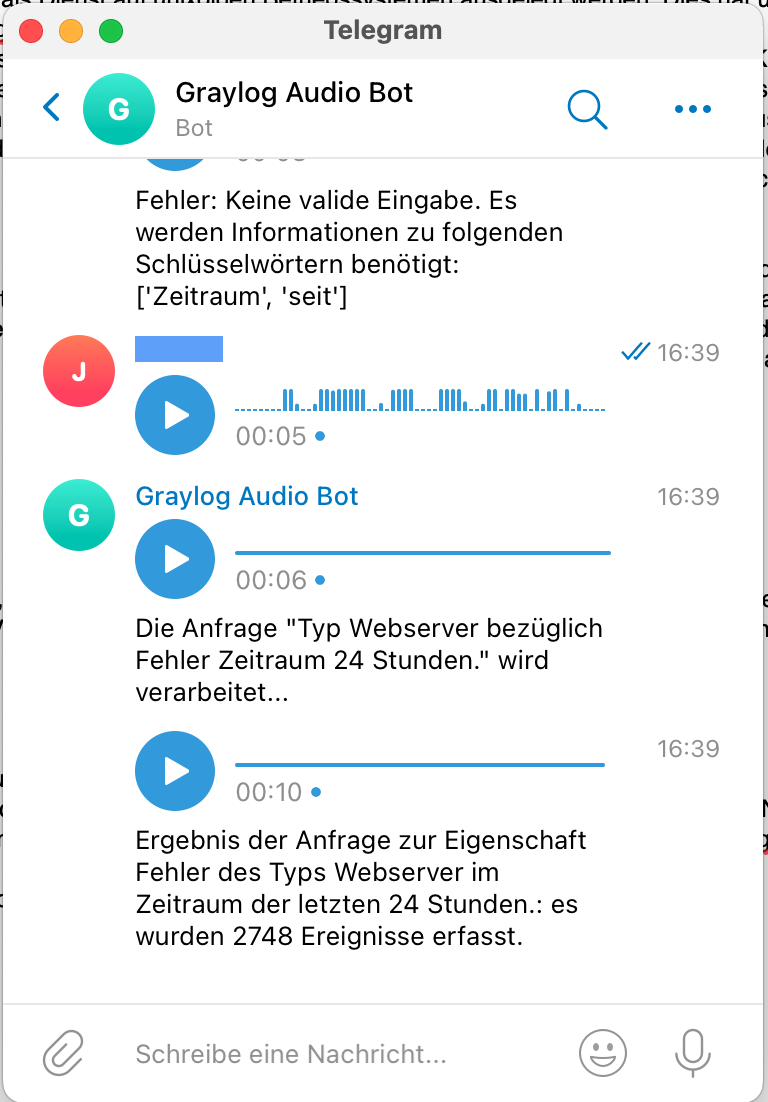
\includegraphics[scale=0.7]{bsp-betrieb}
\caption{Bot beantwortet eine Anfrage in Telegram für macOS.}
\end{figure}

\begin{figure}[h!]
\centering
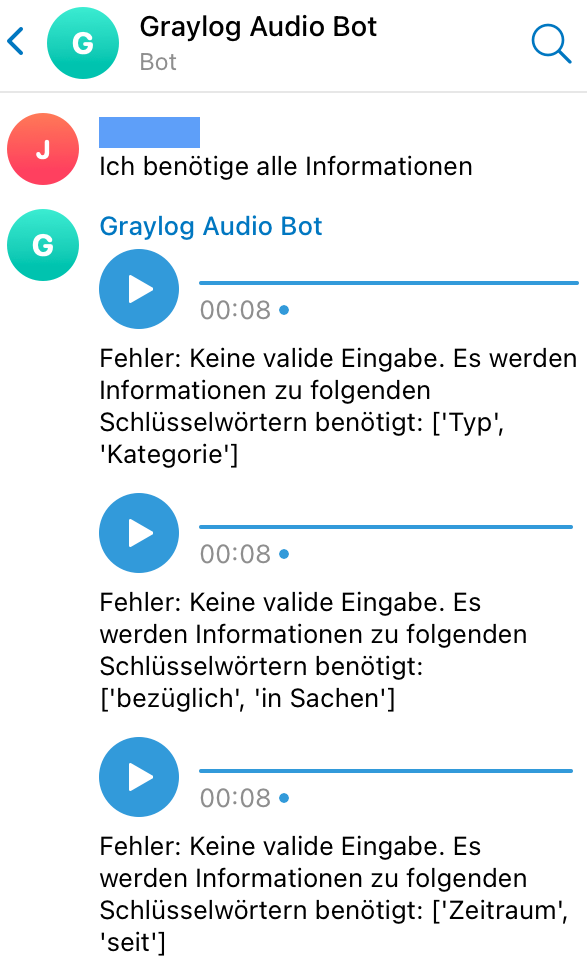
\includegraphics[scale=0.7]{bsp-fehler}
\caption{Bot reagiert auf fehlerhafte Anfrage in Telegram für macOS.}
\end{figure}

\section{Ausblick}



\backmatter
\printbibliography[title=Literaturverzeichnis]
\listoffigures
%\listoftables
\lstlistoflistings
\end{document}
